\documentclass[russian]{llncs}
\usepackage[utf8]{inputenc}
\usepackage[T2A]{fontenc}
\usepackage[final]{graphicx}
\usepackage{epstopdf}
\usepackage[labelsep=period]{caption}
\usepackage[hyphens]{url}
\usepackage{amssymb,amsmath,mathrsfs}
\usepackage[russian,english]{babel}
%\usepackage{multicol}
\usepackage[ruled,vlined,linesnumbered,algo2e]{algorithm2e}
%\usepackage{algorithm}
%\usepackage[noend]{algorithmic}
\usepackage{color}
\usepackage{cmap}
\usepackage{array}
\usepackage{tikz}
\usepackage{pgfplots}
%\usepackage{verbatim}
\usepackage{standalone}

\tolerance=1000
\hbadness=5000
\newcommand{\const}{\mathrm{const}}
\newcommand{\tsum}{\mathop{\textstyle\sum}\limits}
\newcommand{\tprod}{\mathop{\textstyle\prod}\limits}
\newcommand{\cov}{\mathop{\rm cov}\limits}
\newcommand{\Dir}{\mathop{\rm Dir}\nolimits}
\newcommand{\norm}{\mathop{\rm norm}\limits}
\newcommand{\KL}{\mathop{\rm KL}\nolimits}
%\renewcommand{\geq}{\geqslant}
%\renewcommand{\leq}{\leqslant}
\newcommand{\eps}{\varepsilon}
\newcommand{\cond}{\mspace{3mu}{|}\mspace{3mu}}
\newcommand{\Loss}{\mathscr{L}}
\newcommand{\RR}{\mathbb{R}}
\newcommand{\cL}{\mathscr{L}}
\newcommand{\cP}{\mathscr{P}}
\newcommand{\kw}[1]{\textsf{#1}}
\SetKwFor{ForAll}{\textbf{for all}}{}{}

%... and these rows too.
\pgfplotsset{ every non boxed x axis/.append style={x axis line style=-},
     every non boxed y axis/.append style={y axis line style=-}}
\pgfplotsset{compat = 1.3}

\begin{document}
%%Analysis of Images, Social Networks, and Texts
\title{
    BigARTM: Open Source Library for
    Regularized Multimodal %Online Parallel Distributed
    Topic Modeling of Large Collections
}
\author{
    Konstantin Vorontsov\inst{1}
    \and
    Oleksandr Frei\inst{2}
    \and
    Murat Apishev\inst{3}
    \and
    Peter Romov\inst{4}
    \and
    Marina Dudarenko\inst{5}
}
\institute{\noindent
    Dorodnicyn Computing Centre of RAS, MIPT, HSE, Yandex,
    \hfill\email{voron@forecsys.ru}
    \and
    Schlumberger Information Solutions,
    \hfill\email{oleksandr.frei@gmail.com}
    \and
    Lomonosov Moscow State University,
    \hfill\email{great-mel@yandex.ru}
    \and
    Moscow Institute of Physics and Technology,
    Yandex,
    \hfill\email{peter@romov.ru}
    \and
    Lomonosov Moscow State University,
    \hfill\email{m.dudarenko@gmail.com}
}

\maketitle

\begin{abstract}
Probabilistic topic modeling of text collections is a powerful tool for statistical text analysis.
In this paper we announce the \mbox{BigARTM} open source project (\texttt{http://bigartm.org})
for regularized multimodal topic modeling of large collections.
Several experiments on Wikipedia corpus show that BigARTM performs faster and gives better perplexity
comparing to other popular packages, such as Vowpal Wabbit and Gensim.
We~also demonstrate several unique BigARTM features, such as
additive combination of regularizers,
topic sparsing and decorrelation,
multimodal and multilanguage modeling,
which are not available in the other software packages for topic modeling.

\vspace{1em}
\textbf{Keywords:}
    probabilistic topic modeling,
    Probabilistic Latent Sematic Analysis,
    Latent Dirichlet Allocation,
    Additive Regularization of Topic Models,
    stochastic matrix factorization,
    EM-algorithm,
    BigARTM.
\end{abstract}

\section{Introduction}

Topic modeling is a~rapidly developing branch of statistical text analysis~\cite{blei12ptm}.
Topic model reveals a~hidden thematic structure of a~text collection
and finds a~compressed representation of each document in terms of its topics.
Practical applications of topic models include many areas, such as
information retrieval for long-text queries,
%revealing research trends and research fronts,
classification, categorization, summarization and segmentation of texts.
More ideas, models and applications are outlined in the survey~\cite{daud10knowledge}.

From a statistical point of view, a~probabilistic topic model
defines each topic by a~multinomial distribution over words,
and then describes each document with a~multinomial distribution over topics.
From an optimizational point of view,
topic modeling can be considered as a~special case
of approximate stochastic matrix factorization.
To learn a~factorized representation of a~text collection
is an ill-posed problem, which has an infinite set of solutions.
A typical approach in this case is to apply regularization techniques,
which impose problem-specific constrains
and ultimately lead to a~better solution.

Existing works on topic modeling describe hundreds of models, adapted to different situations.
For practitioners, most of the models are too difficult to quickly
understand, compare, combine and embed into applications.
This leads to a~common practice of using only the basic models such as
\emph{Probabilistic Latent Semantic Analysis}, PLSA~\cite{hofmann99plsi} and
\emph{Latent Dirichlet Allocation}, LDA~\cite{blei03latent}.
Some of the difficulties are rooted in Bayesian learning framework,
which is the dominating approach in topic modeling.
Bayesian inference of topic models requires a~laborious mathematical work,
which prevents unification and flexible manipulation of various topic models.
Until now, there was no freely available development tools
to easily design, modify, select, and combine topic models.

In this paper we announce \textbf{the BigARTM open source project} for
regularized multimodal topic modeling of large collections,
\texttt{http://bigartm.org}.
The theory behind BigARTM is based on a non-Bayesian multicriteria approach~---
\emph{Additive Regularization of Topic Models}, ARTM~\cite{voron14dan-eng}.
In~ARTM a~topic model is learned by maximizing a~weighted sum
of the log-likelihood and additional regularization criteria.
The optimization problem is solved by a~general regularized expectation-maximization (EM) algorithm,
which can be applied to an arbitrary combination of regularization criteria.
Many known Bayesian topic models were revisited in terms of ARTM in~\cite{voron14mlj,voron14aist}.
Compared to the Bayesian approach,
ARTM makes it easier to design, infer and combine topic models,
thus reducing the barrier for entering into topic modeling research field.

BigARTM source code is released under the New BSD License, which permits free commercial and non-commercial usage.
The core of the library is written in C++ and is exposed via two equally rich APIs for C++ and Python.
The library is cross-platform and can be built for Linux, Windows and OS X in both 32 and 64 bit configuration.
In our experiments on Wikipedia corpus BigARTM performs better than Vowpal Wabbit LDA and Gensim libraries
in terms of perplexity and runtime.
Comparing to the other libraries BigARTM offers several additional features,
such as regularization and multi-modal topic modeling.

The rest of the paper is organized as follows.
In~section~\ref{sec:Multimodal}
we~introduce a~multimodal topic modeling for documents with additional discrete metadata.
In~section~\ref{sec:Online}
we~generalize the~fast online algorithm~\cite{hoffman10online} to additively regularized multimodal topic models.
In~section~\ref{sec:BigARTM}
we~describe parallel architecture and implementation details of the BigARTM library.
In~section~\ref{sec:Experiments}
we~report results of our experiments on large datasets.
In~section~\ref{sec:Conclusions}
we~discuss advantages, limitations and open problems of BigARTM.

\section{Multimodal regularized topic model}
\label{sec:Multimodal}

%Matching Words and Pictures, MoM-LDA \cite{barnard03matching}
%\cite{virtanen12factorized}
%\cite{roller13multimodal}

Let
$D$ denote a finite set (collection) of texts and
$W^1$ denote a~finite set (vocabulary) of all terms from these texts.
Each term can represent a~single word or a~key phrase.
%Each document ${d\in D}$ is a sequence of terms from the vocabulary~$W^1$.
A document can contain not only words, but also terms of other modalities.
Each modality is defined by a finite set (vocabulary) of terms $W^m$, ${m=1,\dots,M}$.
Examples of not-word modalities are:
authors,
class or category labels,
date-time stamps,
references to/from other documents,
entities mentioned in texts,
objects found in the images associated with the documents,
users that read or downloaded documents,
advertising banners,
etc.

Assume that
each term occurrence in each document refers to some latent topic from a~finite set of topics~$T$.
Text collection is considered to be a sample of triples
$(w_i,d_i,t_i)$,\; ${i=1,\dots,n}$,
drawn independently from a~discrete distribution $p(w,d,t)$ over the finite space $W\times D \times T$,
where ${W=W^1\sqcup\cdots\sqcup W^m}$ is a~disjoint union of the vocabularies across all modalities.
Terms~$w_i$ and documents~$d_i$ are observable variables,
while topics~$t_i$ are latent variables.

Following the idea of Correspondence LDA~\cite{blei03modeling}
and Dependency LDA~\cite{rubin12statistical}
we introduce a topic model for each modality:
\[
    p(w\cond d)
    = \sum_{t\in T} p(w\cond t)\: p(t\cond d)
    = \sum_{t\in T} \phi_{wt} \theta_{td},
    \quad
    d\in D,\; w\in W^m,\; m=1,\dots,M.
\]

The parameters
${\theta_{td}=p(t\cond d)}$ and ${\phi_{wt}=p(w\cond t)}$
form matrices
${\Theta = \bigl( \theta_{td} \bigr)_{T\times D}}$ of \emph{topic probabilities for the documents}, and
${\Phi^m = \bigl( \phi_{wt} \bigr)_{W^m\times T}}$ of \emph{term probabilities for the topics}.
The matrices $\Phi^m$, if stacked vertically, form a ${W\!\!\times\!T}$-matrix~$\Phi$.
Matrices $\Phi^m$ and~$\Theta$ are \emph{stochastic},
that is, their vector-columns represent discrete distributions.
The number of topics~$|T|$ is expected to be much smaller than~$|D|$ and~$|W|$.

To learn parameters $\Phi^m$, $\Theta$ from the multimodal text collection
we maximize the log-likelihood for each $m$-th modality:
\[
    \cL_m (\Phi^m,\Theta) =
    \sum_{d\in D}\sum_{w\in W^m} n_{dw} \ln p(w\cond d)
    \to \max_{\Phi^m,\Theta},
\]
where
$n_{dw}$ is the number of occurrences of the term $w\in W^m$ in the document~$d$.
Note that topic distributions of documents $\Theta$ are common for all modalities.
Following the ARTM approach,
we add a~regularization penalty term $R(\Phi,\Theta)$
and solve a constrained multicriteria optimization problem via scalarization:
\begin{gather}
\label{eq:multimodal}
    \sum_{m=1}^M \tau_m \cL_m (\Phi^m,\Theta)
    + R(\Phi,\Theta)
    \to \max_{\Phi,\Theta};
\\\label{eq:multimodal:norm}
    \sum_{w\in W^m}\!\!\! \phi_{wt} = 1,~
    \phi_{wt}\geq 0;
    \qquad
    \sum_{t\in T} \theta_{td} = 1,~
    \theta_{td}\geq 0.
\end{gather}

The local maximum $(\Phi,\Theta)$
of the problem~\eqref{eq:multimodal},~\eqref{eq:multimodal:norm}
satisfies the following system of equations
with auxiliary variables $p_{tdw} = p(t\cond d,w)$:
\begin{align}
    \label{eq:Estep}
    p_{tdw} &= \norm_{t\in T} \bigl(\phi_{wt}\theta_{td}\bigr);
\\
    \label{eq:Mstep:phi}
    \phi_{wt} &= \norm_{w\in W^m}
        \biggl(
            n_{wt} + \phi_{wt} \frac{\partial R}{\partial \phi_{wt}}
        \biggr);
    \quad
    n_{wt} = \sum_{d\in D} n_{dw} p_{tdw};
\\
    \label{eq:Mstep:theta}
    \theta_{td} &= \norm_{t\in T}
        \biggl(
            n_{td} + \theta_{td} \frac{\partial R}{\partial \theta_{td}}
        \biggr);
    \quad
    n_{td} =
        \sum_{w\in d} \tau_{m(w)} n_{dw} p_{tdw};
        %\sum_{m=1}^M \tau_m \!\!\sum_{w\in W^m}\!\!\! n_{dw} p_{tdw};
\end{align}
where operator
$\norm_{t\in T} x_t = \frac{\max\{x_t,0\}}{\sum\limits_{s\in T} \max\{x_s,0\}}$
transforms a~vector $(x_t)_{t\in T}$ to a~discrete distribution;
$m(w)$~is the modality of the term~$w$, so that $w\in W^{m(w)}$.

The system of equations \eqref{eq:Estep}--\eqref{eq:Mstep:theta}
follows from Karush--Kuhn--Tucker conditions (see Appendix~A for the proof).
It~can be~solved by various numerical methods.
Particularly,
the simple-iteration method is equivalent to the EM algorithm,
which is typically used in~practice.
For single modality (${M=1}$) it gives the regularized EM algorithm
proposed in~\cite{voron14dan-eng}.
With no regularization (${R=0}$) it~corresponds to PLSA~\cite{hofmann99plsi}.

Many Bayesian topic models can be considered
as special cases of ARTM with different regularizers~$R$,
as shown in~\cite{voron14aist,voron14mlj}.
For~example,
LDA~\cite{blei03latent} corresponds to the entropy smoothing regularizer.

Due to the unified framework of additive regularization
BigARTM can build topic models for various applications
simply by choosing a~suitable combination of~regularizers
from a build-in user extendable library.

\section{Online topic modeling}
\label{sec:Online}
%\cite{zhang13sparse}

Following the idea of Online LDA \cite{hoffman10online}
we split the collection~$D$ into batches~$D_b$, ${b=1,\dots,B}$,
and organize EM iterations so that
each document vector $\theta_d$ is~iterated until convergence at a~constant matrix~$\Phi$,
see Algorithm~\ref{alg:Online} and~\ref{alg:ProcessBatch}.
Matrix~$\Phi$ is updated rarely, after all documents from the batch are processed.
For a~large collection
matrix~$\Phi$ often stabilizes after small initial part of the collection.
Therefore a~single pass through the collection might be sufficient to learn a~topic model.
The second pass may be needed for the initial part of the collection.

Algorithm~\ref{alg:Online} does not specify how often to synchronize $\Phi$ matrix
at steps~\ref{alg:sync-begin}--\ref{alg:sync-end}.
It~can be done after every batch or less frequently
(for instance if $\frac{\partial R}{\partial \phi_{wt}}$ takes long time to evaluate).
This flexibility is especially important for concurrent implementation of the algorithm,
where multiple batches are processed in parallel.
In~this case synchronization can be triggered when a fixed number of documents had been processed since the last synchronization.

The online reorganization of the EM iterations
is not necessarily associated with Bayesian inference used in~\cite{hoffman10online}.
Different topic models, from PLSA to multimodal and regularized models,
can be learned by the above online EM algorithm.

\section{BigARTM architecture}
\label{sec:BigARTM}

The main goal for BigARTM architecture is to ensure a constant memory usage regardless of the collection size.
For this reason each $D_b$ batch is stored on disk in a separate file,
and only a limited number of batches is loaded into the main memory at any given time.
The entire $\Theta$ matrix is also never stored in the memory.
As a result, the memory usage stays constant regardless of the size of the collection.

\SetAlgoSkip{}
\begin{algorithm2e}[t]
\caption{Online EM-algorithm for multimodal ARTM}
\label{alg:Online}
\BlankLine
\KwIn{collection $D_b$, discounting factor $\rho\in(0,1]$;}
\KwOut{matrix $\Phi$;}
\BlankLine
initialize $\phi_{wt}$ for all $w \in W$ and $t \in T$\;
$n_{wt} := 0$,~ $\tilde n_{wt} := 0$\;
\ForAll{batches $D_b$, $b = 1,\dots,B$}{
    $\tilde n_{wt} := \tilde n_{wt} + \kw{ProcessBatch}(D_b, \phi_{wt})$\;
    \If{(synchronize)\label{alg:sync-begin}}{
        $n_{wt} := \rho n_{wt} + \tilde n_{dw}$ for all $w \in W$ and $t \in T$\; \label{alg:merging}
        $\phi_{wt} := \norm_{w\in W^m}
            \bigl(
                n_{wt} + \phi_{wt} \frac{\partial R}{\partial \phi_{wt}}
            \bigr)$
        for all $w \in W^m$,\, $m=1,\dots,M$ and $t \in T$\; \label{alg:phi}

        $\tilde n_{wt} := 0$ for all $w \in W$ and $t \in T$\; \label{alg:sync-end}
    }
}
\end{algorithm2e}

\begin{algorithm2e}[t]
\caption{\kw{ProcessBatch}($D_b, \phi_{wt}$)}
\label{alg:ProcessBatch}
\BlankLine
\KwIn{batch $D_b$, matrix $\phi_{wt}$;}
\KwOut{matrix $\tilde n_{wt}$;}
\BlankLine
$\tilde n_{wt} := 0$ for all $w \in W$ and $t \in T$\;
\ForAll{$d \in D_b$}{
	initialize $\theta_{td} := \frac{1}{|T|}$ for all $t \in T$\;
	\Repeat{$\theta_d$ converges}{
        $p_{tdw} := \norm_{t\in T} \bigl(\phi_{wt}\theta_{td}\bigr)$ for all $t \in T$\;
        $n_{td} := \sum_{w\in d} \tau_{m(w)} n_{dw} p_{tdw}$ for all $t \in T$\;
        $\theta_{td} := \norm_{t\in T}
            \bigl(
                n_{td} + \theta_{td} \frac{\partial R}{\partial \theta_{td}}
            \bigr)$ for all $t \in T$\;
	}
	increment $\tilde n_{wt}$ by $n_{dw} p_{tdw}$ for all $w \in d$ and $t \in T$\;
}
\end{algorithm2e}

\paragraph{Concurrency.}
An general rule of concurrency design is to express parallelism at the highest possible level.
For this reason BigARTM implements a concurrent processing of the batches
and keeps a single-threaded code for the $\kw{ProcessBatch}(D_b, \phi_{wt})$ routine.

To split collection into batches and process them concurrently is a common approach,
introduced in AD-LDA algorithm \cite{newman2009distributed}, and
then further developed in PLDA \cite{wang2009plda} and PLDA{+} \cite{liu2011plda+} algorithms.
These algorithms require all concurrent workers to become idle before an update of the $\Phi$ matrix.
Such synchronization step adds a large overhead in the online algorithm where $\Phi$ matrix is updated multiple times on each iteration.
An alternative architecture without the synchronization step is described in \cite{smola2010architecture},
however it mostly targets a distributed cluster environment.
In our work we develop an efficient single-node architecture where all workers benefit from the shared memory space.

\begin{figure}[t]
\begin{centering}
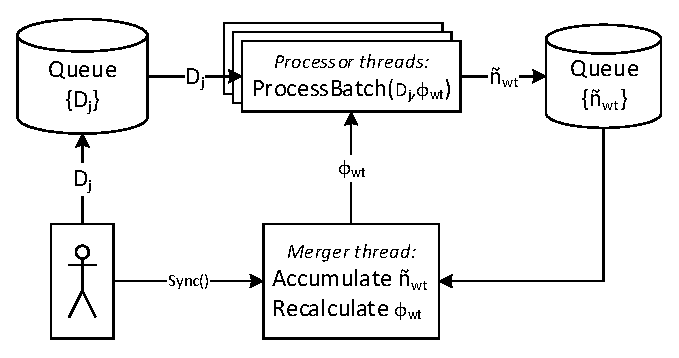
\includegraphics[height=36mm]{diagramm_artm_core.eps}
\caption{Diagram of key BigARTM components}
\label{fig:diagramm_artm_core}
\end{centering}
\end{figure}

To run multiple $\kw{ProcessBatch}$ in parallel the inputs and outputs of this routine are stored in two separate in-memory queues,
locked for push and pop operations with spin locks.
This approach does not add any noticeable synchronization overhead because
both queues only store smart pointers to the actual data objects,
so push and pop operations does not involve copying or relocating big objects in the memory.

Smart pointers are also essential for lifecycle of the $\Phi$ matrix.
This matrix is \emph{read} by all processors threads, and can be \emph{written} at any time by the merger thread.
To update $\Phi$ without pausing all processor threads we keep two copies~--- an \emph{active $\Phi$} and a \emph{background $\Phi$} matrices.
The active matrix is read-only, and is used by the processor threads.
The background matrix is being built in a background by the merger thread
at steps \ref{alg:merging} and~\ref{alg:phi} of Algorithm~\ref{alg:Online},
and once it is ready merger thread marks it as active.
Before processing a new batch the processor thread gets the current active matrix from the merger thread.
This object is passed via shared smart pointer to ensure that processor thread can keep ownership of its $\Phi$ matrix
until the batch is fully processed.
As a result, all processor threads keep running concurrently with the update of $\Phi$ matrix.

Note that all processor threads share the same $\Phi$ matrix,
which means that memory usage stays at constant level regardless of how many cores are used for computation.
Using memory for two copies of the $\Phi$ matrix in our opinion gives a reasonable usage balance between memory and CPU resources.
An~alternative solution with only one $\Phi$ matrix is also possible, but it would require a heavy usage of atomic CPU instructions.
Such operations are very efficient, but still come at a considerable synchronization cost%
\footnote{\url{http://stackoverflow.com/questions/2538070/atomic-operation-cost}},
and using them for all reads and writes of the $\Phi$ matrix would cause a significant performance degradation for merger and processor threads.
Besides, an arbitrary overlap between reads and writes of the $\Phi$ matrix eliminates any possibility of producing a deterministic result.
The design with two copies of the $\Phi$ matrix gives much more control over this
and in certain cases allows BigARTM to behave in a fully deterministic way.

The design with two $\Phi$ matrices only supports a~single merger thread,
and we believe it should handle all $\tilde n_{wt}$ updates coming from many threads.
This is a reasonable assumption because
merging at step~\ref{alg:merging} takes only about $O(|W|\cdot|T|)$ operations to execute, while
$\kw{ProcessBatch}$ takes $O(n |T| I)$ operations,
where
$n$~is the number of non-zero entries in the batch,
$I$~is the average number of inner iterations in $\kw{ProcessBatch}$ routine.
The ratio $n / |W|$ is typically from 100 to 1000 (based on datasets in UCI Bag-Of-Words repository),
and $I$ is $10 \dots 20$, so the ratio safely exceeds the expected number of cores
(up to 32 physical CPU cores in modern workstations, and even 60 cores of the Intel Xeon Phi co-processors).

\paragraph{Data layout.}
BigARTM uses dense single-precision matrices to represent $\Phi$ and~$\Theta$.
Together with the $\Phi$ matrix we store a global dictionary of all terms ${w \in W}$.
This dictionary is implemented as $\kw{std::unordered\_map}$ that maps a string representation of ${w \in W}$
into its integer index in the $\Phi$ matrix.
This dictionary can be extended automatically as more and more batches came through the system.
To achieve this each batch $D_b$ contains a local dictionary $W_b$, listing all terms that occur in the batch.
The $n_{dw}$ elements of the batch are stored as a~sparse CSR matrix (Compressed Sparse Raw format),
where each row correspond to a~document ${d \in D_b}$,
and terms~$w$ run over a~local batch dictionary~$W_b$.

For performance reasons $\Phi$ matrix is stored in column-major order, and $\Theta$ in row-major order.
This layout ensures that $\sum_t \phi_{wt} \theta_{td}$ sum runs on contiguous memory blocks.
In both matrices all values smaller than $10^{-16}$ are always replaced with zero to avoid performance issues with denormalized numbers%
\footnote{\url{http://en.wikipedia.org/wiki/Denormal_number#Performance_issues}}.
%http://stackoverflow.com/questions/9314534/why-does-changing-0-1f-to-0-slow-down-performance-by-10x

\paragraph{Programming interface.}
All functionality of BigARTM is expressed in a set of $\kw{extern C}$ methods.
To input and output complex data structures the API uses Google Protocol Buffers%
\footnote{\url{http://code.google.com/p/protobuf/}}.
This approach makes it easy to integrate BigARTM into any research or production environment,
as almost every modern language has an implementation of Google Protocol Buffers
and a way of calling $\kw{extern C}$ code
($\kw{ctypes}$ module for Python, $\kw{loadlibrary}$ for Matlab, $\kw{PInvoke}$ for C\#, etc).

On top of the $\kw{extern C}$ API BigARTM already has convenient wrappers in C++ and Python.
We are also planning to implement a Java wrapper in the near future.
In addition to the APIs the library also has a simple CLI interface.

BigARTM has built-in libraries of regularizers and quality measures
that can be extended in current implementation only through project recompilation.

\paragraph{Basic tools.}
A careful selection of the programming tools is important for any software project.
This is especially true for BigARTM as its code is written in C++,
a language that by itself offers less functionality comparing to Python, .NET Framework or Java.
To mitigate this we use
various parts of the Boost C++ Libraries,
Google Protocol Buffers for data serialization,
ZeroMQ library for network communication,
and several other libraries.
%This tools are not specific for topic modeling, and should be considered for any scientific library written in C++.

BigARTM uses CMake as a cross-platform build system,
and it successfully builds on Windows, Linux and OS X in 32 and 64 bit configurations.
Building the library require a recent C++ compiler with C++11 support (GNU GCC 4.6.3, clang 3.4 or Visual Studio 2012 or newer),
and Boost Libraries 1.46.1 or newer. All the other third-parties are included in BigARTM repository.

We also use free online services
to store source code (\url{https://github.com}),
to host online documentation (\url{https://readthedocs.org}) and
to run automated continuous integration builds (\url{http://travis-ci.org}).

\section{Experiments}
\label{sec:Experiments}

In this section we evaluate the runtime performance and the algorithmic quality of \mbox{BigARTM}
against two popular software packages~---
Gensim~\cite{rehurek_lrec}
%\footnote{\url{http://radimrehurek.com/gensim/}}
and Vowpal Wabbit%
\footnote{\url{https://github.com/JohnLangford/vowpal_wabbit/}}.
We also demonstrate some of the unique BigARTM features, such as
combining regularizers and multi-language topic modeling via multimodality,
which are not available in the other software packages.

All three libraries (VW.LDA, Gensim and BigARTM) work out-of-core,
e.\,g. they are designed to process data that is too large to fit into a computer's main memory at one time.
This allowed us to benchmark on a fairly large collection --- 3.7 million articles from the English Wikipedia%
\footnote{\url{http://dumps.wikimedia.org/enwiki/20141208/}}.
The conversion to bag-of-words was done with $\kw{gensim.make\_wikicorpus}$ script%
\footnote{\url{https://github.com/piskvorky/gensim/tree/develop/gensim/scripts/}},
which excludes all non-article pages (such as category, file, template, user pages, etc),
and also pages that contain less than $50$~words.
The dictionary is formed by all words that occur in at least 20~documents,
but no more than in $10\%$ documents in the collection.
The resulting dictionary was caped at $|W| = 100\,000$ most frequent words.

Both Gensim and VW.LDA represents the resulting topic model as Dirichlet distribution over $\Phi$ and $\Theta$ matrices:
$\vec{\theta}_{d} \sim \text{Dir}(\vec{\gamma}_d)$ and
$\vec{\phi}_{t} \sim \text{Dir}(\vec{\lambda}_t)$.
On~contrary, BigARTM outputs a non-probabilistic matrices $\Phi$ and $\Theta$.
To~compare the perplexity we take the mean or the mode of the posterior distributions:
\begin{align*}
    \phi^{\mathrm{mean}}_{wt} &= \norm_{w\in W} \lambda_{wt}, &
	\theta^{\mathrm{mean}}_{td} &= \norm_{t\in T} \gamma_{td};
\\
    \phi^{\mathrm{mode}}_{wt} &= \norm_{w\in W} (\lambda_{wt}-1), &
	\theta^{\mathrm{mode}}_{td} &= \norm_{t\in T} (\gamma_{td}-1).
\end{align*}
The perplexity measure is defined as
\begin{equation}
    \label{eq:perplexity}
    \mathscr{P}(D, p) =
        %\exp\left(- \frac{1}{n} L(\Phi, \Theta) \right) =
        \exp \biggl( - \frac{1}{n} \sum_{d \in D} \sum_{w \in d} n_{dw} \ln p(w \cond d) \biggr).
\end{equation}

\paragraph{Comparison to existing software packages.}

%There is no article to quote for VW, check http://www.research.rutgers.edu/~lihong/pub/Qin13Efficient.pdf - they use a footnote to quote VW
The \emph{Vowpal Wabbit (VW)} is a library
of online algorithms that cover a wide range of machine learning problems. %, not specifically limited to topic modeling.
For~topic modeling VW has the VW.LDA algorithm, based on the Online Variational Bayes LDA \cite{hoffman10online}.
VW.LDA is neither multi-core nor distributed,
but an effective single-threaded implementation in C++ made it one of the fastest tools for topic modeling.% within single computing node.

The \emph{Gensim} library specifically targets the area of topic modeling and matrix factorization.
It has two LDA implementations --- LdaModel and LdaMulticore,
both based on the same algorithm as VW.LDA (Online Variational Bayes LDA~\cite{hoffman10online}).
Gensim is entirely written in Python. Its high performance is achieved through the usage of NumPy library,
built over low-level BLAS libraries (such as Intel MKL, ATLAS, or OpenBLAS).
In LdaModel all batches are processed sequentially, and the concurrency happens entirely within NumPy. % (in numpy.dot, numpy.sum and other Level1 BLAS operations).
In LdaMulticore the workflow is similar to BigARTM --- several batches are processed concurrently, and there is a single aggregation thread that asynchronously merges the results.

\begin{table}[t]
	\caption{
        The comparison of BigARTM with VW.LDA and Gensim.
        \emph{Train time} is the time for model training,
        \emph{inference} is the time for calculation of $\theta_d$ of $100\,000$ held-out documents,
        \emph{perplexity} is calculated according to \eqref{eq:perplexity} on held-out documents.
    }
	\label{tab:libraries_comparison}
    \vskip-2ex\centering\tabcolsep=8pt
	\begin{tabular}[t]{l|c|rrrr}
	\hline
	& & & & \multicolumn{2}{c}{perplexity} \\
	library & procs & train time & inference & mode & mean \\
	\hline
	BigARTM +smoothing & 1 & 62 min & 127 sec & \multicolumn{2}{c}{4000} \\
	Gensim LDA & 1 & 369 min & 395 sec & 4213 & 4161  \\
	Vowpal Wabbit LDA & 1 & 73 min & 120 sec & 4061 & 4108 \\
	\hline
	BigARTM +smoothing & 4 & 13 min & 33 sec & \multicolumn{2}{c}{4061}  \\
	Gensim LDA-Multicore & 4 & 60 min & 222 sec & 4055 & 4111  \\	
	\hline
	BigARTM +smoothing & 8 & 8 min & 24 sec & \multicolumn{2}{c}{4304}  \\
	Gensim LDA-Multicore & 8 & 57 min & 224 sec & 4379 & 4455 \\
	\hline
	\end{tabular}
\end{table}

\begin{figure}[t]
	\centering
	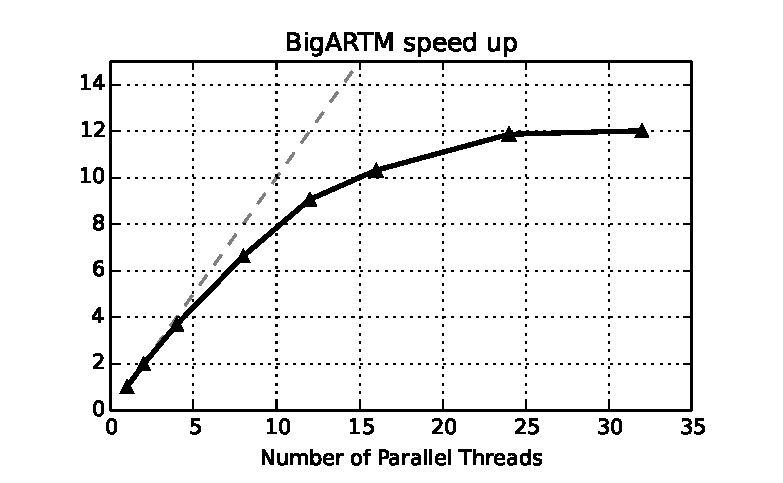
\includegraphics[height=35mm]{speedup_bigartm.eps}
	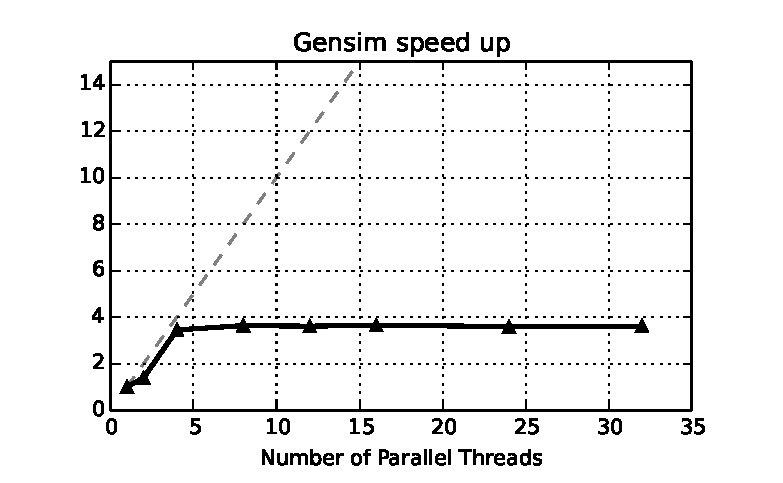
\includegraphics[height=35mm]{speedup_gensim.eps}
	\caption{Speed up for BigARTM (left chart) and Gensim (right chart)}
	\label{fig:bigartm_speedup}
\end{figure}

Each run in our experiment performs one pass over the Wikipedia corpus and produces a~model with $|T|=100$ topics.
The runtime is reported for an Intel-based CPU with 16 physical cores with hyper-threading.
The collection was split into batches with $10 000$ documents each
(\texttt{chunksize} in Gensim, \texttt{minibatch} in VW.LDA).
The update rule in online algorithm used
${\rho = (b + \tau_0)^{-0.5}}$,
where $b$ is the number of batches processed so far,
and $\tau_0$ is an a constant offset parameter introduced in \cite{hoffman10online},
in~our experiment ${\tau_0 = 64}$.
Updates were performed after each batch in non-parallel runs, and after $P$ batches when running in $P$ threads.
LDA priors were fixed as
${\alpha = 0.1}$,\, ${\beta = 0.1}$,
so that
$\vec{\theta}_d \sim \text{Dir}(\alpha)$,\,
$\vec{\phi}_t \sim \text{Dir}(\beta)$.

Table\;\ref{tab:libraries_comparison} compares the performance of VW.LDA, Gensim, and BigARTM.

Fig.\;\ref{fig:bigartm_speedup} compares BigARTM and Gensim speedup depending on the number of CPU threads
for Amazon AWS~c3.8xlarge with 32~cores,
Gensim~\mbox{0.10.3} under Python~\mbox{2.7},
and the parameter of LDA-Multicore $\kw{workers}=\kw{nProcessors}-1$.

%{\color{red}ToDo: discussions.}

\paragraph{Experiments with combination of regularizers.}

BigARTM has a~built-in library of regularizers, which can be used in any combination.
In~the following experiment we combine three regularizers:
sparsing of~$\phi_{t}$~distributions,
sparsing of~$\theta_{d}$~distributions, and
pairwise decorrelation of~$\phi_{t}$ distributions.
This combination helps to improve several quality measures without significant loss of perplexity,
according to~experiments on the offline implementation of ARTM~\cite{voron14aist}.
The goal of our experiment is to show that this remains true
for the online implementation in BigARTM.
We~use the following built-in quality measures:
the hold-out perplexity,
the sparsity of $\Phi$ and $\Theta$ matrices, and
the characteristics of topic lexical kernels (size, purity, and contrast) averaged across all topics.

\begin{table}[t]
    \caption{Comparison of LDA and ARTM models.
        Quality measures:
        $\mathcal{P}_{10k}$, $\mathcal{P}_{100k}$ --- hold-out perplexity on 10K and 100K documents sets,
        $\mathcal{S}_{\Phi}$, $\mathcal{S}_{\Theta}$ --- sparsity of $\Phi$ and $\Theta$ matrices (in \%),
        $\mathcal{K}_{s}$, $\mathcal{K}_{p}$, $\mathcal{K}_{c}$ --- average topic kernel size, purity and contrast respectively.}
    \label{tab:model_comparison}
    \centering\vskip-2ex\tabcolsep=8pt
    \begin{tabular}[t]{l|rrrrrrr}
    \hline
    Model & $\mathcal{P}_{10k}$ & $\mathcal{P}_{100k}$ &  $\mathcal{S}_{\Phi}$ & $\mathcal{S}_{\Theta}$ &  $\mathcal{K}_{s}$ & $\mathcal{K}_{p}$ &  $\mathcal{K}_{c}$ \\
    \hline
    LDA              & 3499 & 3827 & 0.0  & 0.0  & 931  & 0.535 & 0.516 \\
    ARTM             & 3592 & 3944 & 96.3 & 80.5 & 1135 & 0.810 & 0.732 \\
    \hline
    \end{tabular}
\end{table}

\begin{figure}[t]
\begin{tabular}{cc}
\documentclass{standalone}

\usepackage{tikz}
\usepackage{pgfplots}
\usepackage{verbatim}

\pgfplotsset{ every non boxed x axis/.append style={x axis line style=-},
     every non boxed y axis/.append style={y axis line style=-}}     
\pgfplotsset{compat = 1.9}

\begin{document}
\scriptsize

\begin{tikzpicture}[remember picture, baseline=0pt, scale = 0.8]
    \begin{axis}[
        ylabel shift = -3 pt,
        width=7cm,
        height=5cm,
        axis lines=left,
        ymajorgrids=true,
        xmajorgrids=true,
        ymin = 0, ymax = 100000,
        major grid style={draw=lightgray},
        ylabel={\scriptsize $\mathrm{\bf Perplexity}$},
        scaled x ticks = false,                    
        ]
    \addplot[smooth,line width=0.4mm] plot coordinates {
		(80000, 93308)
		(210000, 69748)
		(350000, 40293)
		(470000, 33250)
		(600000, 24970)
		(750000, 20488)
		(860000, 17735)
		(1020000, 15461)
		(1130000, 14215)
		(1250000, 12848)
		(1390000, 11726)
		(1500000, 11023)
		(1640000, 10443)
		(1750000, 10016)
		(1870000, 9555)
		(2000000, 9128)
		(2130000, 8829)
		(2260000, 8527)
		(2360000, 8300)
		(2480000, 8071)
		(2630000, 7858)
		(2740000, 7713)
		(2860000, 7511)
		(2990000, 7345)
		(3100000, 7227)
		(3260000, 7084)
		(3360000, 6996)
		(3508494, 6889)
		(3658494, 6781)
		(3718494, 6723)
    }; \label{perplexityPlsa}
    
    \addplot[smooth,line width=0.2mm] plot coordinates {
		(80000, 93470)
		(210000, 85201)
		(340000, 52457)
		(470000, 35692)
		(600000, 27265)
		(750000, 21531)
		(860000, 19200)
		(1020000, 16156)
		(1130000, 14820)
		(1250000, 13445)
		(1390000, 12148)
		(1500000, 11393)
		(1640000, 10815)
		(1760000, 10255)
		(1870000, 9812)
		(2010000, 9290)
		(2140000, 8958)
		(2250000, 8663)
		(2350000, 8418)
		(2480000, 8149)
		(2620000, 7908)
		(2730000, 7750)
		(2850000, 7536)
		(2990000, 7303)
		(3100000, 7178)
		(3260000, 7016)
		(3360000, 6926)
		(3518494, 6786)
		(3658494, 6670)
		(3718494, 6623)    
    }; \label{perplexityLda}
    \end{axis}
    
    \begin{axis}[
    	ylabel shift = -7 pt,
        width=7cm,
        height=5cm,
        axis lines=left,
        axis x line*=top,
        xtick=\empty,
        axis y line*=right,
        ymin = 0, ymax = 100,
        ylabel near ticks,             
        ylabel={\scriptsize $\mathrm{\bf Sparsity}$},
        legend columns=3, 
        legend style={
            text width=5.5em,
            text height=1.5ex,
            text depth=.5ex,        
        	draw=none,
            /tikz/column 3/.style={
                column sep=0pt,
            },
            at={(axis description cs:1.14,-0.14)}
        },
        every axis legend/.append style={nodes={right}},
        ]
    \addlegendimage{black}        
    \addlegendimage{dashed, black} 
    \addlegendimage{dotted, black}
    \addlegendimage{/pgfplots/refstyle=perplexityPlsa}\addlegendentry{\scriptsize $\mathrm{\:\; Perplexity}$} 
    \addplot[dashed,line width=0.4mm] plot coordinates {
		(80000, 2)
		(210000, 71)
		(350000, 67)
		(470000, 68)
		(600000, 72)
		(750000, 75)
		(860000, 78)
		(1020000, 80)
		(1130000, 82)
		(1250000, 83)
		(1390000, 84)
		(1500000, 85)
		(1640000, 89)
		(1750000, 90)
		(1870000, 90)
		(2000000, 91)
		(2130000, 91)
		(2260000, 92)
		(2360000, 92)
		(2480000, 93)
		(2630000, 93)
		(2740000, 93)
		(2860000, 93)
		(2990000, 94)
		(3100000, 94)
		(3260000, 94)
		(3360000, 94)
		(3508494, 94)
		(3658494, 94)
		(3718494, 95)
    };           
    \addlegendentry{\scriptsize $\mathrm{\hphantom{A}\hphantom{A}Phi}$}

    \addplot[dashed,line width=0.2mm] plot coordinates {
		(80000, 2)
		(210000, 0)
		(340000, 0)
		(470000, 0)
		(600000, 0)
		(750000, 0)
		(860000, 0)
		(1020000, 0)
		(1130000, 0)
		(1250000, 0)
		(1390000, 0)
		(1500000, 0)
		(1640000, 0)
		(1760000, 0)
		(1870000, 0)
		(2010000, 0)
		(2140000, 0)
		(2250000, 0)
		(2350000, 0)
		(2480000, 0)
		(2620000, 0)
		(2730000, 0)
		(2850000, 0)
		(2990000, 0)
		(3100000, 0)
		(3260000, 0)
		(3360000, 0)
		(3518494, 0)
		(3658494, 0)
		(3718494, 0)
    };
    
    \addplot[dotted,line width=0.4mm] plot coordinates {
		(80000, 0)
		(210000, 0)
		(350000, 3)
		(470000, 25)
		(600000, 42)
		(750000, 52)
		(860000, 58)
		(1020000, 63)
		(1130000, 66)
		(1250000, 69)
		(1390000, 71)
		(1500000, 73)
		(1640000, 75)
		(1750000, 76)
		(1870000, 77)
		(2000000, 78)
		(2130000, 79)
		(2260000, 80)
		(2360000, 80)
		(2480000, 81)
		(2630000, 82)
		(2740000, 82)
		(2860000, 83)
		(2990000, 83)
		(3100000, 83)
		(3260000, 84)
		(3360000, 84)
		(3508494, 84)
		(3658494, 85)
		(3718494, 85)
    };         
    \addlegendentry{\scriptsize $\mathrm{\hphantom{A}\hphantom{A}Theta}$}  
    
    \addplot[dotted,line width=0.2mm] plot coordinates {
		(80000, 0.000000)
		(210000, 0.000000)
		(340000, 0.010000)
		(470000, 0.010000)
		(600000, 0.030000)
		(750000, 0.140000)
		(860000, 0.340000)
		(1020000, 0.700000)
		(1130000, 0.880000)
		(1250000, 0.800000)
		(1390000, 0.720000)
		(1500000, 0.650000)
		(1640000, 0.610000)
		(1760000, 0.560000)
		(1870000, 0.530000)
		(2010000, 0.490000)
		(2140000, 0.460000)
		(2250000, 0.440000)
		(2350000, 0.420000)
		(2480000, 0.400000)
		(2620000, 0.380000)
		(2730000, 0.360000)
		(2850000, 0.350000)
		(2990000, 0.330000)
		(3100000, 0.320000)
		(3260000, 0.300000)
		(3360000, 0.290000)
		(3518494, 0.280000)
		(3658494, 0.270000)
		(3718494, 0.270000)	
    };
    \end{axis}
\end{tikzpicture}
\normalsize

\end{document}
&
\documentclass{standalone}

\usepackage{tikz}
\usepackage{pgfplots}
\usepackage{verbatim}

\pgfplotsset{ every non boxed x axis/.append style={x axis line style=-},
     every non boxed y axis/.append style={y axis line style=-}}     
\pgfplotsset{compat = 1.3}

\begin{document}
\scriptsize

\begin{tikzpicture}[remember picture, baseline=0pt, scale = 0.8]
    \begin{axis}[
        ylabel shift = -2 pt,
        width=7cm,
        height=5cm,
        axis lines=left,
        ytick = {0, 200, 400, 600, 800, 1000},
        ymajorgrids=true,
        xmajorgrids=true,        
		scaled y ticks = true,
		scaled y ticks=base 10:-3,
        ymin = 0, ymax = 1100,
        major grid style={draw=lightgray},
        ylabel={\scriptsize $\mathrm{\bf Kernel~size}$},
        scaled x ticks = false,                   
        ]
    \addplot[smooth,line width=0.4mm] plot coordinates {
		(80000, 7)
		(210000, 471)
		(350000, 635)
		(470000, 741)
		(600000, 873)
		(750000, 957)
		(860000, 1000)
		(1020000, 1029)
		(1130000, 1044)
		(1250000, 1055)
		(1390000, 1062)
		(1500000, 1066)
		(1640000, 1064)
		(1750000, 1066)
		(1870000, 1065)
		(2000000, 1062)
		(2130000, 1057)
		(2260000, 1054)
		(2360000, 1049)
		(2480000, 1046)
		(2630000, 1042)
		(2740000, 1038)
		(2860000, 1036)
		(2990000, 1032)
		(3100000, 1030)
		(3260000, 1026)
		(3360000, 1023)
		(3508494, 1020)
		(3658494, 1017)
		(3718494, 1014)
    }; \label{kernelSizePlsa}
    
    \addplot[smooth,line width=0.2mm] plot coordinates {
		(80000, 7)
		(210000, 4)
		(340000, 20)
		(470000, 67)
		(600000, 162)
		(750000, 335)
		(860000, 433)
		(1020000, 480)
		(1130000, 539)
		(1250000, 615)
		(1390000, 679)
		(1500000, 717)
		(1640000, 745)
		(1760000, 775)
		(1870000, 790)
		(2010000, 824)
		(2140000, 837)
		(2250000, 859)
		(2350000, 867)
		(2480000, 880)
		(2620000, 894)
		(2730000, 895)
		(2850000, 903)
		(2990000, 920)
		(3100000, 927)
		(3260000, 936)
		(3360000, 937)
		(3518494, 945)
		(3658494, 954)
		(3718494, 952)    
    }; \label{kernelSizeLda}
    \end{axis}
    
    \begin{axis}[
    	ylabel shift = -4 pt,
        width=7cm,
        height=5cm,
        axis lines=left,
        axis x line*=top,
        xtick=\empty,
        axis y line*=right,
        ymin = 0, ymax = 1.1,
        ylabel near ticks,             
        ylabel={\scriptsize $\mathrm{\bf Purity~and~contrast}$},
        legend columns=3, 
        legend style={
            text width=4.5em,
            text height=1.5ex,
            text depth=.5ex,
        	draw=none,
            /tikz/column 3/.style={
                column sep=0pt,
            },
            at={(axis description cs:0.98,-0.14)}
        },        
        ]
    \addlegendimage{smooth, black}        
    \addlegendimage{dashed, black} 
    \addlegendimage{dotted, black}
    \addlegendimage{/pgfplots/refstyle=perplexityPlsa}\addlegendentry{\scriptsize $\mathrm{\hphantom{A}Size}$} 
    \addplot[dashed,line width=0.4mm] plot coordinates {
		(80000, 0.000000)
		(210000, 0.006000)
		(350000, 0.013000)
		(470000, 0.030000)
		(600000, 0.065000)
		(750000, 0.109000)
		(860000, 0.153000)
		(1020000, 0.199000)
		(1130000, 0.237000)
		(1250000, 0.266000)
		(1390000, 0.301000)
		(1500000, 0.331000)
		(1640000, 0.384000)
		(1750000, 0.402000)
		(1870000, 0.409000)
		(2000000, 0.427000)
		(2130000, 0.445000)
		(2260000, 0.455000)
		(2360000, 0.469000)
		(2480000, 0.481000)
		(2630000, 0.491000)
		(2740000, 0.503000)
		(2860000, 0.505000)
		(2990000, 0.513000)
		(3100000, 0.521000)
		(3260000, 0.527000)
		(3360000, 0.536000)
		(3508494, 0.542000)
		(3658494, 0.547000)
		(3718494, 0.553000)
    };           
    \addlegendentry{\scriptsize $\mathrm{\hphantom{A}Purity}$}

    \addplot[dashed,line width=0.2mm] plot coordinates {
		(80000, 0.000000)
		(210000, 0.001000)
		(340000, 0.002000)
		(470000, 0.010000)
		(600000, 0.023000)
		(750000, 0.051000)
		(860000, 0.073000)
		(1020000, 0.104000)
		(1130000, 0.125000)
		(1250000, 0.151000)
		(1390000, 0.177000)
		(1500000, 0.201000)
		(1640000, 0.220000)
		(1760000, 0.238000)
		(1870000, 0.250000)
		(2010000, 0.270000)
		(2140000, 0.287000)
		(2250000, 0.297000)
		(2350000, 0.309000)
		(2480000, 0.323000)
		(2620000, 0.335000)
		(2730000, 0.343000)
		(2850000, 0.354000)
		(2990000, 0.363000)
		(3100000, 0.369000)
		(3260000, 0.379000)
		(3360000, 0.384000)
		(3518494, 0.393000)
		(3658494, 0.400000)
		(3718494, 0.403000)
    };
    
    \addplot[dotted,line width=0.4mm] plot coordinates {
		(80000, 0.313000)
		(210000, 0.559000)
		(350000, 0.501000)
		(470000, 0.527000)
		(600000, 0.540000)
		(750000, 0.557000)
		(860000, 0.572000)
		(1020000, 0.585000)
		(1130000, 0.596000)
		(1250000, 0.605000)
		(1390000, 0.614000)
		(1500000, 0.622000)
		(1640000, 0.646000)
		(1750000, 0.651000)
		(1870000, 0.654000)
		(2000000, 0.660000)
		(2130000, 0.667000)
		(2260000, 0.671000)
		(2360000, 0.676000)
		(2480000, 0.680000)
		(2630000, 0.683000)
		(2740000, 0.687000)
		(2860000, 0.689000)
		(2990000, 0.691000)
		(3100000, 0.693000)
		(3260000, 0.696000)
		(3360000, 0.698000)
		(3508494, 0.700000)
		(3658494, 0.702000)
		(3718494, 0.704000)
    };         
    \addlegendentry{\scriptsize $\mathrm{\hphantom{A}Contrast}$}  
    
    \addplot[dotted,line width=0.2mm] plot coordinates {
		(80000, 0.308000)
		(210000, 0.303000)
		(340000, 0.328000)
		(470000, 0.337000)
		(600000, 0.350000)
		(750000, 0.373000)
		(860000, 0.386000)
		(1020000, 0.390000)
		(1130000, 0.400000)
		(1250000, 0.413000)
		(1390000, 0.427000)
		(1500000, 0.436000)
		(1640000, 0.443000)
		(1760000, 0.451000)
		(1870000, 0.456000)
		(2010000, 0.466000)
		(2140000, 0.471000)
		(2250000, 0.477000)
		(2350000, 0.480000)
		(2480000, 0.485000)
		(2620000, 0.489000)
		(2730000, 0.491000)
		(2850000, 0.494000)
		(2990000, 0.499000)
		(3100000, 0.502000)
		(3260000, 0.506000)
		(3360000, 0.507000)
		(3518494, 0.510000)
		(3658494, 0.513000)
		(3718494, 0.513000)	
    };
    \end{axis}
\end{tikzpicture}
\normalsize
\end{document}
\end{tabular}
\caption{Comparison of LDA (thin) and ARTM (bold) models. The number of processed documents is shown along the X~axis.}
\label{fig:comparison_plot}
\end{figure}

Table \ref{tab:model_comparison} compares the results of additive combination of regularizers (ARTM) and the usual LDA model.
Figure \ref{fig:comparison_plot} presents quality measures as functions of the number of processed documents.
The left chart shows perplexity and sparsity of $\Phi$, $\Theta$ matrices, and
the right chart shows average lexical kernel measures.

%{\color{red}ToDo: discussions.}

\paragraph{Experiments on multi-language Wikipedia.}

To~show how BigARTM works with multimodal datasets we prepared a text corpus
containing all English and Russian Wikipedia articles with mutual interlanguage links.
We represent each linked pair of articles
as a single multi-language document with~two modalities, one modality for each language.
That is how our multi-language collection acts as a multimodal document collection.

The dump of Russian articles%
\footnote{\url{http://dumps.wikimedia.org/ruwiki/20141203/}}
had been processed following the same technique as we previously used in experiments on English Wikipedia.
Russian words were lemmatized with Yandex MyStem~3.0%
\footnote{\url{https://tech.yandex.ru/mystem/}}.
To further reduce the dictionary we only keep words
that appear in no less than 20~documents, but no~more than in~10\% of~documents in the collection.
The resulting collection contains 216175~pairs of Russian--English articles, with combined dictionary
of 196749 words (43\% Russian, 57\% English words).

We build multi-language model with 400~topics.
They cover a wide range of themes such as science, architecture, history, culture, technologies, army, different countries.
%Most of them can be easily interpreted.
All $400$ topics were reviewed by an independent assessor,
and he successfully interpreted all except four topics.

Table \ref{tab:top10words} shows top 10 words for four randomly selected topics.
Top words in these topics are clearly consistent between Russian and English languages.
The Russian part of last topic contains some English words such as
``Windows'' or ``Server'' because it is common to use them in Russian texts without translation.

\begin{table}[t!]
	\caption{
        Top 10 words with $p(w\cond t)$ probabilities (in~\%) from two-language topic model,
        based on Russian and English Wikipedia articles with mutual interlanguage links.}
	\label{tab:top10words}
	\centering\tabcolsep=3pt%\small
	\footnotesize
    \begin{tabular}{|lr|lr||lr|lr|}	
    	\hline
    	\multicolumn{4}{|c||}{\textbf{Topic~68}} & \multicolumn{4}{c|}{\textbf{Topic~79}\rule{0pt}{3ex}} \\
    	\hline
    	research & 4.56 & институт & 6.03 & goals & 4.48 & матч & 6.02 \\
    	technology & 3.14 & университет & 3.35 & league & 3.99 & игрок & 5.56 \\
    	engineering & 2.63 & программа & 3.17 & club & 3.76 &  сборная & 4.51 \\
    	institute & 2.37 & учебный & 2.75 & season & 3.49 & фк & 3.25 \\
    	science & 1.97 & технический & 2.70 & scored & 2.72 & против & 3.20 \\
    	program & 1.60 & технология & 2.30 & cup & 2.57 & клуб & 3.14 \\
    	education & 1.44 & научный & 1.76 & goal & 2.48 & футболист & 2.67 \\
    	campus & 1.43 & исследование & 1.67 & apps & 1.74 & гол & 2.65 \\
    	management & 1.38 & наука & 1.64 & debut & 1.69 & забивать & 2.53 \\
    	programs & 1.36 & образование & 1.47 & match & 1.67 & команда & 2.14 \\
    	\hline
    	\multicolumn{4}{|c||}{\textbf{Topic~88}} &     \multicolumn{4}{c|}{\textbf{Topic~251}\rule{0pt}{3ex}}  \\
    	\hline
        opera & 7.36 & опера & 7.82 & windows & 8.00 & windows & 6.05 \\
    	conductor & 1.69 & оперный & 3.13 & microsoft & 4.03 & microsoft & 3.76 \\
    	orchestra & 1.14 & дирижер & 2.82 & server & 2.93 & версия & 1.86 \\
    	wagner & 0.97 & певец & 1.65 & software & 1.38 & приложение & 1.86 \\
    	soprano & 0.78 & певица & 1.51 & user & 1.03 & сервер & 1.63 \\
    	performance & 0.78 & театр & 1.14 & security & 0.92 & server & 1.54 \\
    	mozart & 0.74 & партия & 1.05 & mitchell & 0.82 & программный & 1.08 \\
    	sang & 0.70 & сопрано & 0.97 & oracle & 0.82 &  пользователь & 1.04 \\
    	singing & 0.69 & вагнер & 0.90 & enterprise & 0.78 & обеспечение & 1.02 \\
    	operas & 0.68 & оркестр & 0.82 & users & 0.78 & система & 0.96 \\
    	\hline
	\end{tabular}
\end{table}


%There are many efficient LDA implementations for single node processing.
%In this section we discuss Vowpal Wabbit LDA \cite{vwlda} and Gensim \cite{gensim} as most popular ones.
%At first we review their technical and algorithmic features and compare them with solutions applied to our library.
%In addition we explain the reasons why we refused to integrate ARTM into these implementations.
%Then we compare the results of experiments on these libraries and BigARTM.
%
%\paragraph{Vowpal Wabbit LDA.} LDA in Vowpal Wabbit is online, as other algorithms in this library.
%It bases on Online Variational Bayes LDA described by Matthew Hoffman in \cite{hoffman10online}.
%Online VB LDA in Vowpal Wabbit supports single-threaded documents processing, it's neither a multi-core nor distributed.
%Nevertheless, effective implementation in C++ without STL and good scalability of the algorithm
%made VW.LDA one of the fastest tools for topic modeling within single computing node.
%However, it's not very comfortable: Vowpal Wabbit LDA doesn't have user API and launches from CLI.
%This implies the limitations of possibilities to tune the parameters of topic model and to control its quality.
%
%Online algorithm and C++ usage are the common features of BigARTM and VW.LDA
%\footnote{But we also use STL ? Boost libraries}. Also both of libraries are cross-platform.
%But there are more differences than similarities. BigARTM accelerates processing by using multithreaded computing.
%Library capabilities and user API are much richer. API allows to tune almost all phases of algorithm.
%At the same time, it's also possible to use library from CLI as in VW.LDA, if necessary.
%
%\paragraph{Gensim.} Cross-platform and written on Python, library Gensim has two different LDA implementations.
%The first one is LdaModel, it's almost a clone of Online VB LDA.
%The high performance of data processing is achieved through the usage of NumPy library, built over low-level BLAS library
%\footnote{Intel MKL, ATLAS etc.}. The second implementation is LdaMulticore.
%It also bases on Online VB LDA, but supports multi-core processing. LdaMulticore creates a workflow per core,
%which processes it's own part of documents. In addition, it creates a general aggregating stream, that merges
%asynchronously the results, recieved from workflows. In this way, LdaModel uses several cores to process one batch of documents,
%and in LdaMulticore each core processes it's own batch. Gensim has a comfortable enough user interface.
%Moreover, it has a capability to find topic distributions for new documents using pre-built topic model.
%
%BigARTM and Gensim.LdaMulticore proceed multithreaded data processing in the same way.
%BigARTM also can find topic distributions for new documents. But our library supports multimodal models.
%And it's more productive. In the following experiments we show,
%that BigARTM's scalability is higher, than LdaMulticore's one.
%
%\paragraph{Motivation.} BigARTM's idea is to create a versatile tool for topic modeling that meets several criteria:
%
%\begin{itemize}
%	\item Online data processing.
%	\item ARTM support with possibility to add new regularizers and functionals of quality.
%	\item Permanent monitoring of topic model during learning.
%	\item A capability to be integrated in other programming languages.
%	\item Efficient parallel data processing.
%	\item Rich and flexible user API.
%	\item Cross-platform.
%\end{itemize}
%Some of this conditions exclude the possibility of using VW.LDA or Gensim as the base of ARTM.
%Vowpal Wabbit is a common library of online algorithms, which contain LDA as one of the working modes.
%It's impossible to control the state of the model or to influence it during the learning process.
%As we noted above, there's no user API in VW.LDA.
%In addtition, the source code of the library is difficult for modification and support.
%
%The key reason we refused to implement ARTM in Gensim is that it's written on Python.
%This language doesn't provide the possibility to be integrated into other languages easy.
%And C++ does. Moreover, we consider Gensim.LdaMulticore to be not very efficient. This question is discussed below.
%
%BigARTM satisfies all of the given criteria. It's effective, easily extensible due to the plug-ins,
%supports user interfaces for different languages. As we noted above, the library can learn several topic models simultaneously,
%apply different regularization strategies. Also it allows to correct parameters
%of the regularizers and models during the learning process and unload any intermediate and final information about the models.

\section{Conclusions}
\label{sec:Conclusions}

\mbox{BigARTM} in an open source project for parallel online topic modeling of large text collections.
It~provides a~high flexibility for various applications due to
multimodality and additive combinations of regularizers.
\mbox{BigARTM} architecture has a~rich potential.
Current components can be reused in a~distributed solution that runs on cluster.
Further improvement of single-node can be achieved by offloading batch processing into GPU.

\bigskip
\subsubsection*{Acknowledgements.}
    The work was supported by~the Russian Foundation for Basic Research grants 14-07-00847, 14-07-00908, 14-07-31176
    and by~Skolkovo Institute of Science and Technology (project 081-R).


%%%%%%%%%%%%%%%%%%%%%%%%%%%%%%%%%%%%%%%%%%%%%%%%%%%%%%%%%%%%%%%%%%%%%%%%%%%%
%\bibliographystyle{splncs03}
%\bibliography{MachLearn}

\begin{thebibliography}{10}
%\providecommand{\url}[1]{\texttt{#1}}
%\providecommand{\urlprefix}{URL }

\bibitem{blei12ptm}
Blei, D.M.: Probabilistic topic models. Communications of the ACM  55(4),
  77--84 (2012)

\bibitem{blei03modeling}
Blei, D.M., Jordan, M.I.: Modeling annotated data. In: Proceedings of the 26th
  Annual International ACM SIGIR Conference on Research and Development in
  Informaion Retrieval. pp. 127--134. ACM, New York, NY, USA (2003)

\bibitem{blei03latent}
Blei, D.M., Ng, A.Y., Jordan, M.I.: Latent {Dirichlet} allocation. Journal of
  Machine Learning Research  3,  993--1022 (2003)

\bibitem{daud10knowledge}
Daud, A., Li, J., Zhou, L., Muhammad, F.: Knowledge discovery through directed
  probabilistic topic models: a survey. Frontiers of Computer Science in China
  4(2),  280--301 (2010)

\bibitem{hoffman10online}
Hoffman, M.D., Blei, D.M., Bach, F.R.: Online learning for latent dirichlet
  allocation. In: NIPS. pp. 856--864. Curran Associates, Inc. (2010)

\bibitem{hofmann99plsi}
Hofmann, T.: Probabilistic latent semantic indexing. In: Proceedings of the
  22nd annual international ACM SIGIR conference on Research and development in
  information retrieval. pp. 50--57. ACM, New York, NY, USA (1999)

\bibitem{liu2011plda+}
Liu, Z., Zhang, Y., Chang, E.Y., Sun, M.: PLDA+: Parallel latent dirichlet
  allocation with data placement and pipeline processing. ACM Transactions on
  Intelligent Systems and Technology (TIST)  2(3), ~26 (2011)

\bibitem{newman2009distributed}
Newman, D., Asuncion, A., Smyth, P., Welling, M.: Distributed algorithms for
  topic models. The Journal of Machine Learning Research  10,  1801--1828
  (2009)

\bibitem{rehurek_lrec}
{\v R}eh{\r u}{\v r}ek, R., Sojka, P.: {Software Framework for Topic Modelling
  with Large Corpora}. In: {Proceedings of the LREC 2010 Workshop on New
  Challenges for NLP Frameworks}. pp. 45--50. ELRA, Valletta, Malta (May 2010).
  %\url{http://is.muni.cz/publication/884893/en}

\bibitem{rubin12statistical}
Rubin, T.N., Chambers, A., Smyth, P., Steyvers, M.: Statistical topic models
  for multi-label document classification. Machine Learning  88(1-2),  157--208
  (2012)

\bibitem{smola2010architecture}
Smola, A., Narayanamurthy, S.: An architecture for parallel topic models.
  Proceedings of the VLDB Endowment  3(1-2),  703--710 (2010)

\bibitem{voron14dan-eng}
Vorontsov, K.V.: Additive regularization for topic models of text collections.
  Doklady Mathematics  89(3),  301--304 (2014)

\bibitem{voron14mlj}
Vorontsov, K.V., Potapenko, A.A.: Additive regularization of topic models.
  Machine Learning, Special Issue on Data Analysis and Intelligent Optimization
   (2014)

\bibitem{voron14aist}
Vorontsov, K.V., Potapenko, A.A.: Tutorial on probabilistic topic modeling:
  Additive regularization for stochastic matrix factorization. In: AIST'2014,
  Analysis of Images, Social networks and Texts. vol. 436, pp. 29--46. Springer
  International Publishing Switzerland, Communications in Computer and
  Information Science (CCIS) (2014)

\bibitem{wang2009plda}
Wang, Y., Bai, H., Stanton, M., Chen, W.Y., Chang, E.Y.: PLDA: Parallel latent
  dirichlet allocation for large-scale applications. In: Algorithmic Aspects in
  Information and Management, pp. 301--314. Springer (2009)

\end{thebibliography}
%%%%%%%%%%%%%%%%%%%%%%%%%%%%%%%%%%%%%%%%%%%%%%%%%%%%%%%%%%%%%%%%%%%%%%%%%%%%

\newpage
\section*{Appendix A}

Consider the system of equations \eqref{eq:Estep}--\eqref{eq:Mstep:theta}.

Topic~$t$ is called \emph{regular} for the modality~$m$
if ${n_{wt} + \phi_{wt} \frac{\partial R}{\partial \phi_{wt}} > 0}$
for at least one term ${w\in W^m}$.
If~the~reverse inequality holds for all ${w\in W^m}$ then
topic~$t$ is called \emph{irregular}.

Document~$d$ is called \emph{regular}
if ${n_{td} + \theta_{td} \frac{\partial R}{\partial \theta_{td}} > 0}$
for at least one topic ${t\in T}$.
If~the reverse inequality holds for all ${t\in T}$ then
document~$d$ is called \emph{irregular}.

\begin{theorem}
\label{th:multimodal}
    If the function $R(\Phi,\Theta)$ is continuously differentiable
    and $(\Phi,\Theta)$ is the local maximum
    of the problem~\eqref{eq:multimodal},~\eqref{eq:multimodal:norm}
    then for any regular topic-modality pair $(t,m)$ and any regular document~$d$
    the system of equations \eqref{eq:Estep}--\eqref{eq:Mstep:theta} holds.
\end{theorem}

\begin{note}
    If a~topic~$t$ is irregular
    then the $t$-th vector-column in matrix~$\Phi^m$ equals zero
    and can not represent a~discrete distribution.
    This means that topic~$t$ for the modality~$m$ must be excluded from the model.
    This mechanism is useful for irrelevant topics elimination and determining the number of topics.
\end{note}
\begin{note}
    If a~documents~$d$ is irregular
    then the $d$-th vector-column in matrix~$\Theta$ equals zero
    and can not represent a~discrete distribution.
    This means that document~$d$ must be excluded from the model.
    For example, a~document may be too short or irrelevant to the given collection.
\end{note}

\begin{proof}
    For the local minimum $\Phi^m,\Theta$
    of the problem~\eqref{eq:multimodal},~\eqref{eq:multimodal:norm}
    the Karush--Kuhn--Tucker (KKT) conditions can be written as follows:
    %(conditions with respect to $\theta_{td}$ are analogous):
    \begin{gather*}
        \sum_{d} n_{dw} \frac{\theta_{td}}{p(w\cond d)} + \frac{\partial R}{\partial \phi_{wt}}
        = \lambda_t - \lambda_{wt};
        \quad
        \lambda_{wt}\geq 0;
        \quad
        \lambda_{wt}\phi_{wt} = 0;
    \\
        \sum_{m} \tau_m \!\!\sum_{w\in W^m}\!\! n_{dw} \frac{\phi_{wt}}{p(w\cond d)} + \frac{\partial R}{\partial \theta_{td}}
        = \mu_d - \mu_{td};
        \quad
        \mu_{td}\geq 0;
        \quad
        \mu_{td}\theta_{td} = 0;
    \end{gather*}
    where $\lambda_t$, $\lambda_{wt}$, $\mu_d$, $\mu_{td}$
    are KKT multipliers for normalization and nonnegativity constrains.

    Let us multiply
    both sides of the first equation by~$\phi_{wt}$,
    both sides of the second equation by~$\theta_{td}$,
    and reveal the auxiliary variable~$p_{tdw}$ from~\eqref{eq:Estep}
    in~the~left-hand side of both equations.
    Then we sum
    the right-hand side of the first equation over~$d$,
    the right-hand side of the second equation over~$t$:
    \begin{gather*}
        \phi_{wt} \lambda_t
        =
        \sum_{d}
        n_{dw} \frac{\phi_{wt}\theta_{td}}{p(w\cond d)}
        + \phi_{wt} \frac{\partial R}{\partial \phi_{wt}}
        =
        n_{wt} + \phi_{wt} \frac{\partial R}{\partial \phi_{wt}};
    \\
        \theta_{td} \mu_{d}
        =
        \sum_{m} \tau_m \!\!\sum_{w\in W^m}\!\!
        n_{dw} \frac{\phi_{wt}\theta_{td}}{p(w\cond d)}
        + \theta_{td} \frac{\partial R}{\partial \theta_{td}}
        =
        n_{td} + \theta_{td} \frac{\partial R}{\partial \theta_{td}}.
    \end{gather*}

    An~assumption that $\lambda_t\leq 0$ contradicts the regularity condition for the $(t,m)$ pair.
    Then ${\lambda_t>0}$.
    Either ${\phi_{wt}= 0}$ or both sides of the first equation are positive.
    Combining these two cases in one formula, we write:
    \begin{equation}
    \label{eq:in-theorem-1:phi}
        \phi_{wt} \lambda_t
        =
        \max\biggl\{
        n_{wt} + \phi_{wt} \frac{\partial R}{\partial \phi_{wt}}, 0
        \biggr\}.
    \end{equation}
    Analogously,
    an~assumption that $\mu_d\leq 0$ contradicts the regularity condition for the document~$d$.
    Then ${\mu_d>0}$.
    Either ${\theta_{td}= 0}$ or both sides of the second equation are positive,
    consequently,
    \begin{equation}
    \label{eq:in-theorem-1:theta}
        \theta_{td} \mu_d
        =
        \max\biggl\{
        n_{td} + \theta_{td} \frac{\partial R}{\partial \theta_{td}}, 0
        \biggr\}.
    \end{equation}

    Let us sum
    both sides of~the first equation over all~${w\in W^m}$,
    then
    both sides of~the second equation over all~${t\in T}$:
    \begin{gather}
    \label{eq:in-theorem-2:phi}
        \lambda_t
        =
        \sum_{w\in W^m}
        \max\biggl\{
        n_{wt} + \phi_{wt} \frac{\partial R}{\partial \phi_{wt}}, 0
        \biggr\};
    \\
    \label{eq:in-theorem-2:theta}
        \mu_d
        =
        \sum_{t\in T}
        \max\biggl\{
        n_{td} + \theta_{td} \frac{\partial R}{\partial \theta_{td}}, 0
        \biggr\}.
    \end{gather}

    Finally,
    we obtain~\eqref{eq:Mstep:phi} by expressing $\phi_{wt}$ from~\eqref{eq:in-theorem-1:phi} and \eqref{eq:in-theorem-2:phi}.

    Analogously,
    we obtain~\eqref{eq:Mstep:theta} by expressing $\theta_{td}$ from~\eqref{eq:in-theorem-1:theta} and \eqref{eq:in-theorem-2:theta}.
    \qed
\end{proof}

\end{document}

